\section{CHƯƠNG 1: KẾT QUẢ THỰC HIỆN TRONG TUẦN 8 (18/05/2026 - 24/05/2026)}

\subsection{Tổng quan}

Trong tuần thứ 8 của dự án (18/05/2026 -- 24/05/2026), các công việc
chính tập trung vào việc hoàn thiện các chức năng còn thiếu trên màn hình
Board và Card Detail, đồng thời tiến hành kiểm thử tổng thể hệ thống để
đánh giá tính ổn định trước khi triển khai lên môi trường Staging.

Các hạng mục đã hoàn thành bao gồm:

\begin{itemize}
    \item Hoàn thiện chức năng thêm thành viên vào Board.
    \item Hoàn thiện Card Detail Modal với các chức năng Due Date,
    Checklist và Card Member.
    \item Hiển thị trạng thái Due Date trực tiếp trên Card.
    \item Tích hợp đầy đủ CRUD API cho Checklist và Checklist Item.
    \item Tích hợp chức năng gán thành viên vào Card.
\end{itemize}

\textbf{Tóm tắt kết quả tuần 8}

\begin{table}[H]
\centering
\begin{tabular}{|p{4cm}|p{9cm}|}
\hline
\textbf{Hạng mục} & \textbf{Kết quả đạt được} \\
\hline
Board Member Management &
Hoàn thiện chức năng thêm thành viên vào Board và đồng bộ dữ liệu với backend. \\
\hline
Due Date Management &
Triển khai thiết lập Due Date và hiển thị trạng thái trên Card. \\
\hline
Checklist Management &
Hoàn thiện CRUD Checklist và Checklist Item. \\
\hline
Card Member Management &
Hoàn thiện chức năng gán và hủy gán thành viên cho Card. \\
\hline
System Testing &
Kiểm thử các luồng chức năng chính và ghi nhận các lỗi còn tồn tại. \\
\hline
\end{tabular}
\end{table}
\clearpage

% -------------------------------------------------------
\subsection{Board Member Management}

\begin{itemize}
    \item Triển khai chức năng quản lý thành viên trong Board.
    \item Thiết kế giao diện hiển thị danh sách thành viên hiện tại của Board.
    \item Thiết kế giao diện thêm thành viên từ danh sách thành viên thuộc Workspace.
    \item Tích hợp API:
\end{itemize}

\begin{verbatim}
GET /api/v1/board-members?boardId=...&search=...

POST /api/v1/boards-members
BODY: {
  "userIds": [
    "string"
  ],
  "boardId": "string",
  "roleId": 1073741824,
  "createdBy": "string"
}
\end{verbatim}

\begin{itemize}
    \item Đồng bộ dữ liệu Board sau khi thêm thành viên thành công.
    \item Xử lý trạng thái loading và thông báo lỗi khi request thất bại.
\end{itemize}

% TODO: Chèn ảnh màn hình Board Member
\begin{figure}[H]
\centering
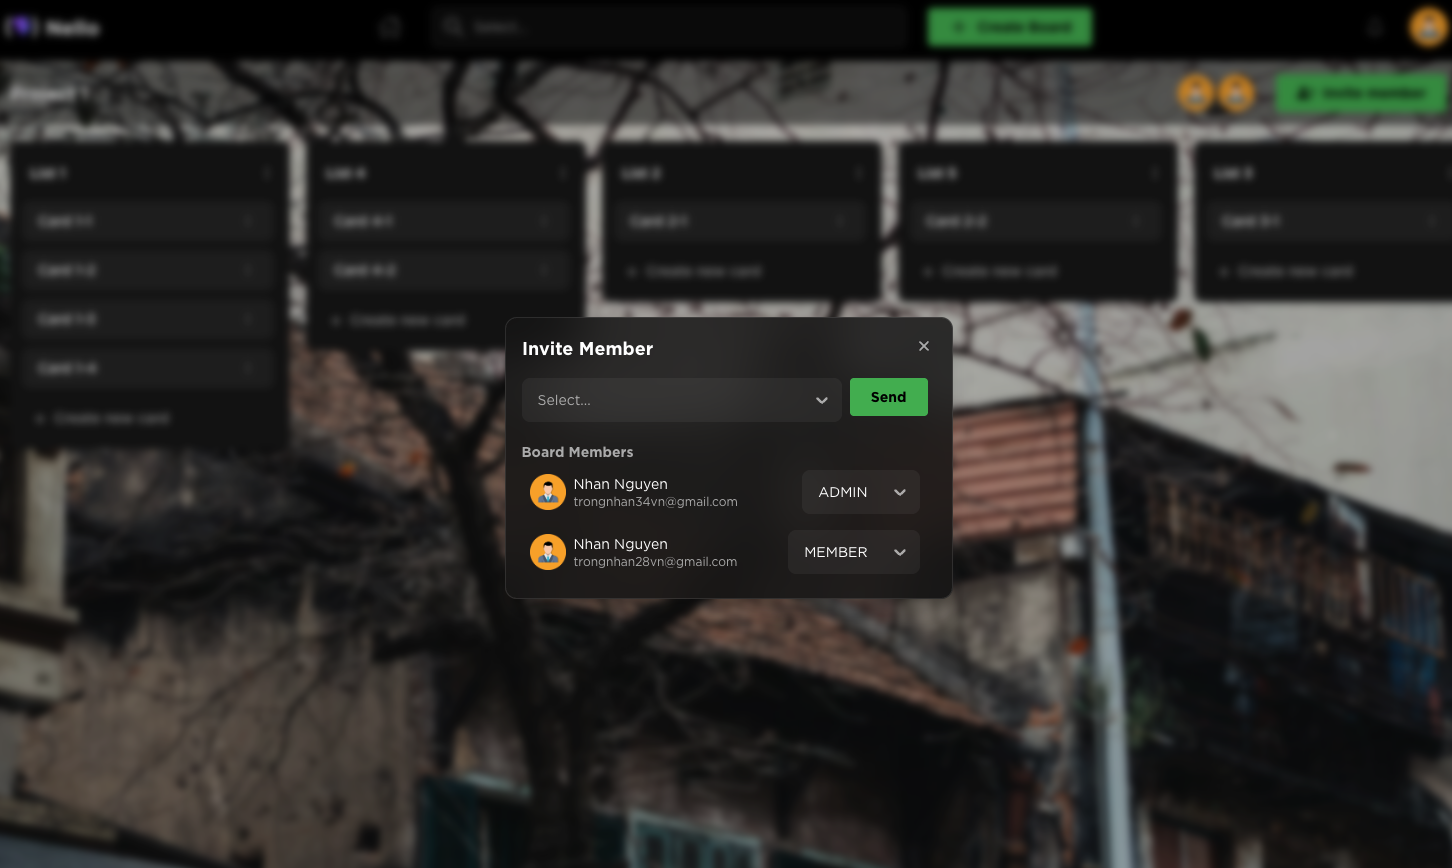
\includegraphics[width=0.9\textwidth]{images/W8_CreateBoardMemberSuccess.png}
\caption{Board Member Management}
\end{figure}

% -------------------------------------------------------
\subsection{Card Detail Enhancement}

\subsubsection{Due Date}

Đã triển khai chức năng quản lý thời hạn hoàn thành công việc (Due Date)
trong Card Detail Modal.

\begin{itemize}
    \item Lựa chọn và cập nhật Due Date bằng Date Picker.
    \item Tích hợp API:
\end{itemize}

\begin{verbatim}
PATCH /api/v1/cards/:id
BODY {
  "id": "string",
  "title": "string",
  "description": "string",
  "startDate": "string",
  "dueDate": "string",
  "position": "string",
  "listId": "string",
  "updatedBy": "string",
  "completed": true,
  "isCompleted": true
}
\end{verbatim}

\begin{itemize}
    \item Hiển thị trạng thái Due Date trực tiếp trên Card.
    \item Hỗ trợ nhận biết công việc sắp đến hạn hoặc đã quá hạn.
\end{itemize}

% TODO: Chèn ảnh Due Date
\begin{figure}[H]
\centering
 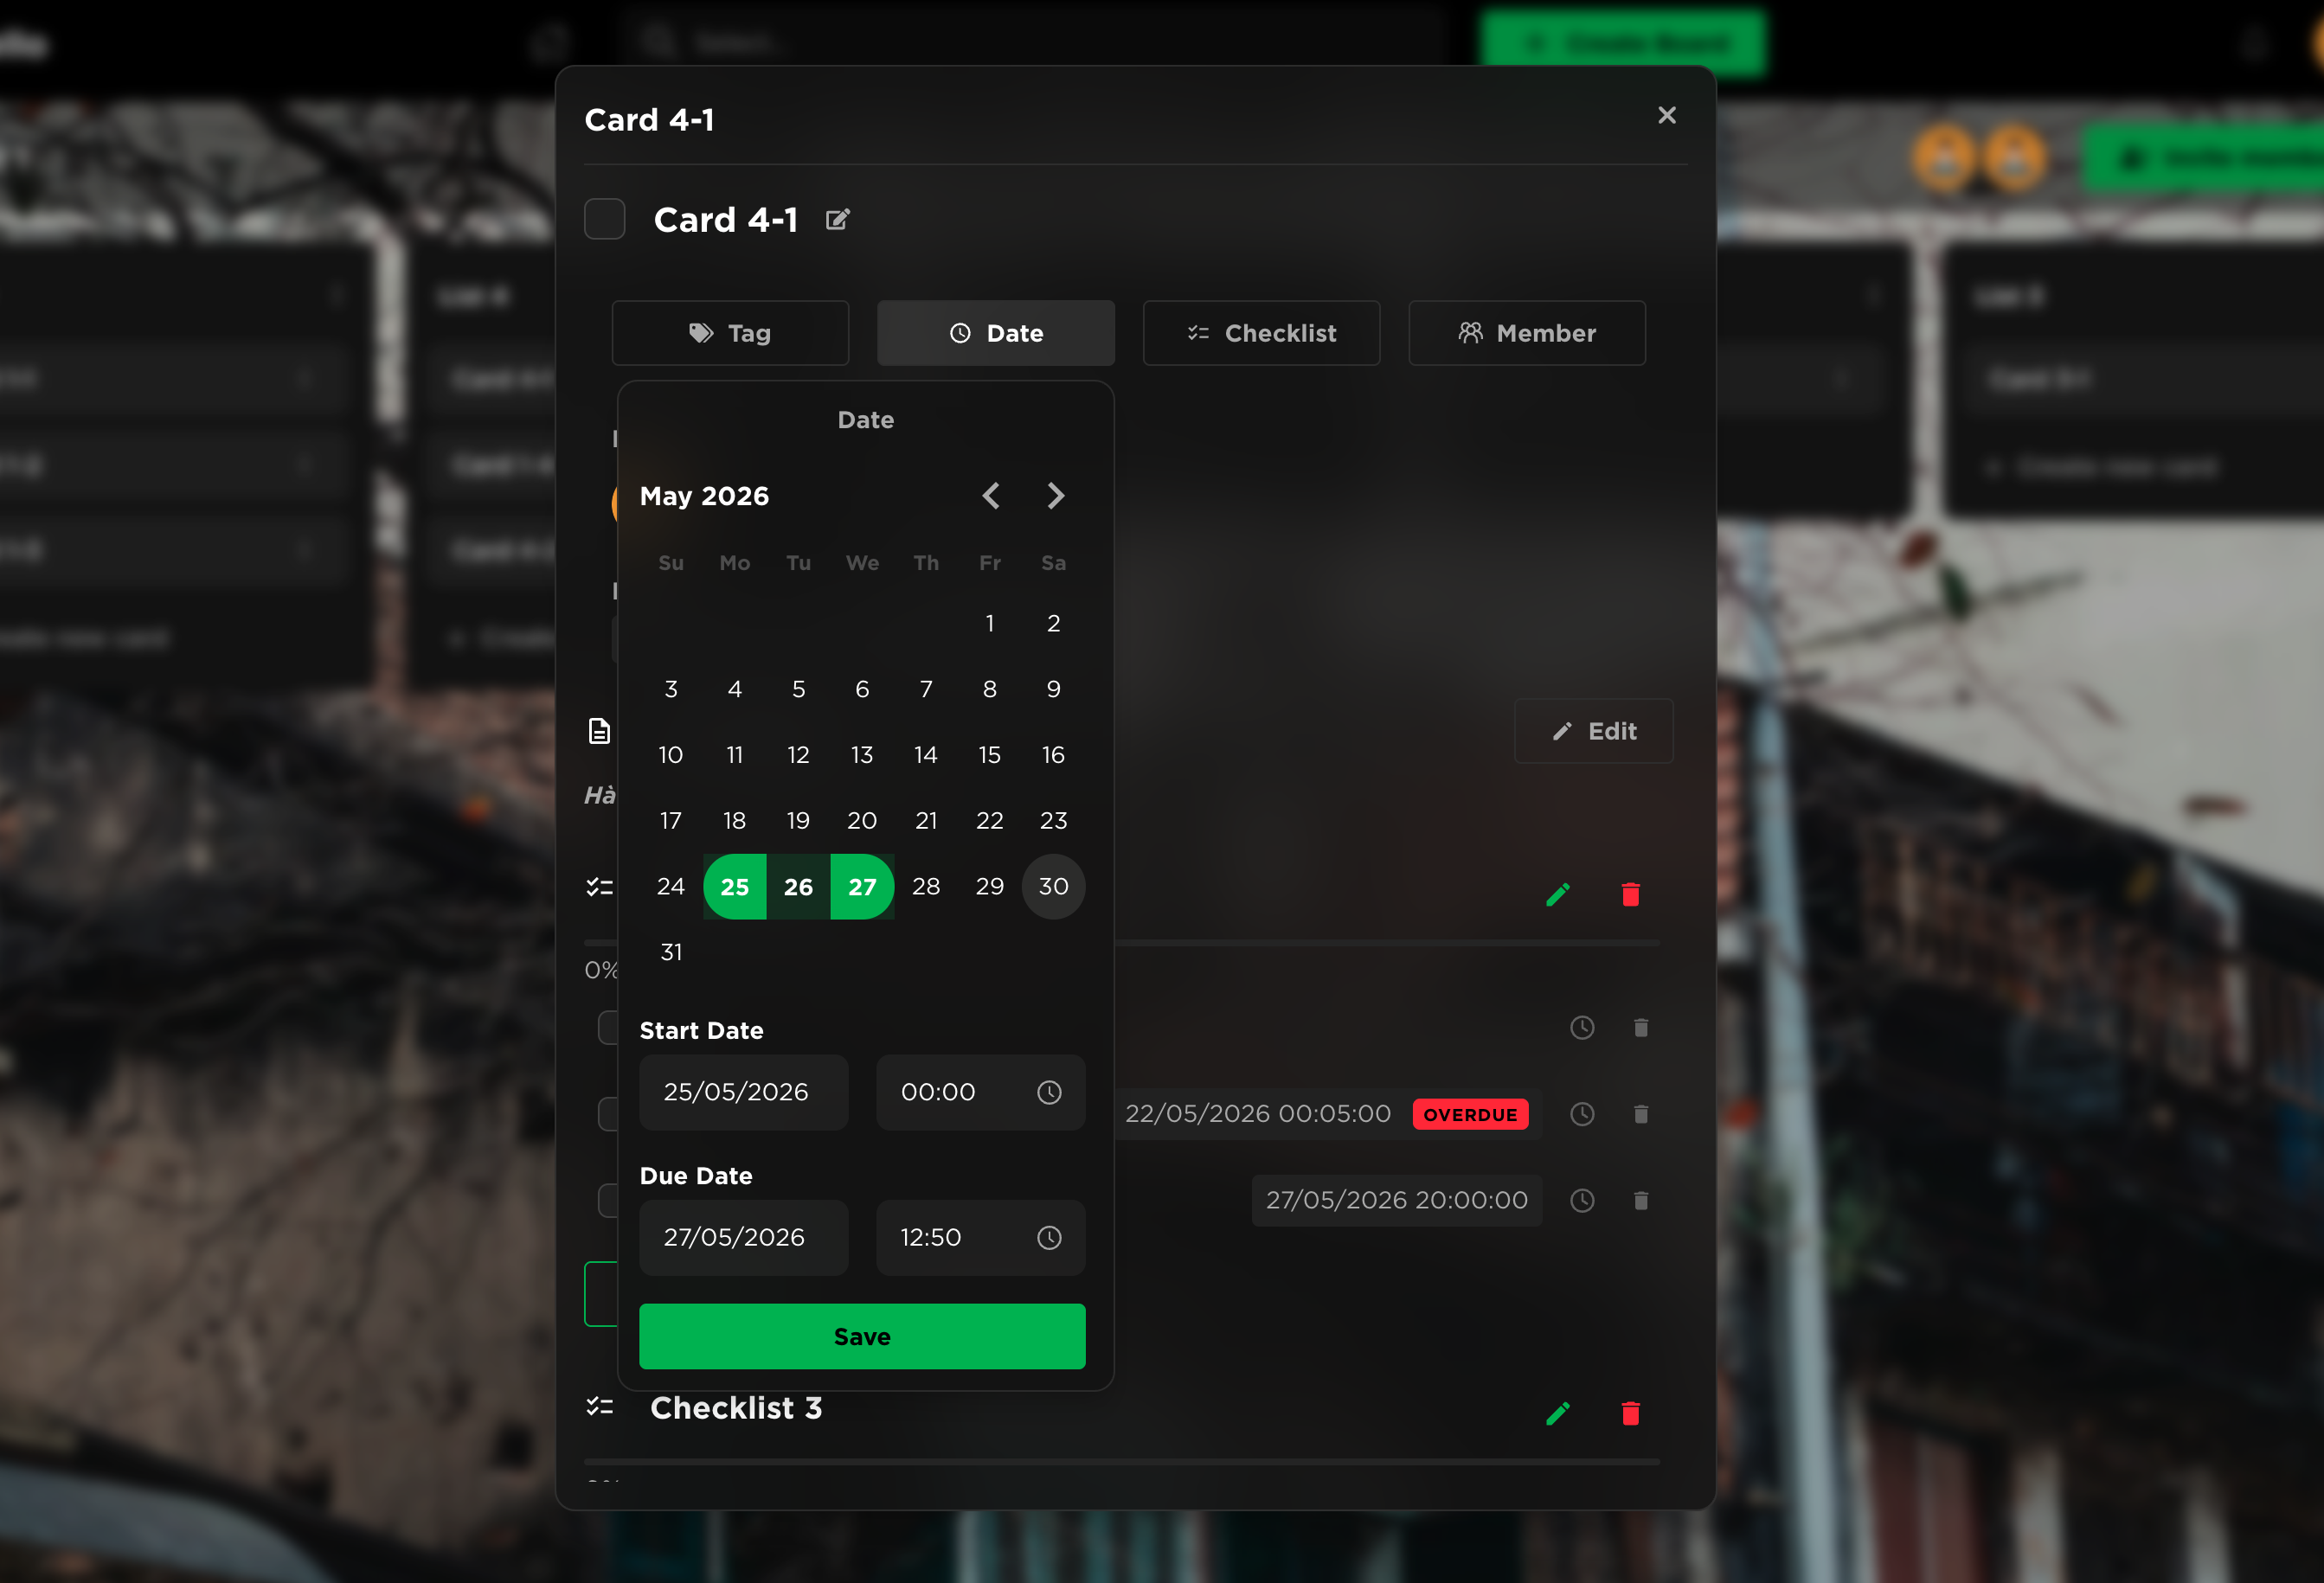
\includegraphics[width=0.9\textwidth]{images/W8_DueDate.png}
\caption{Due Date Management}
\end{figure}

\subsubsection{Checklist}

Đã hoàn thiện đầy đủ chức năng quản lý Checklist trong Card Detail.

Các API đã được tích hợp:

\begin{verbatim}
POST   /api/v1/checklists
PATCH  /api/v1/checklists/:id
DELETE /api/v1/checklists/:id

POST   /api/v1/checklist-items
PATCH  /api/v1/checklist-items/:id
DELETE /api/v1/checklist-items/:id
\end{verbatim}

Các chức năng hỗ trợ:

\begin{itemize}
    \item Tạo Checklist.
    \item Cập nhật Checklist.
    \item Xóa Checklist.
    \item Thêm Checklist Item.
    \item Đánh dấu hoàn thành hoặc chưa hoàn thành.
    \item Xóa Checklist Item.
    \item Hiển thị tiến độ thực hiện bằng Progress Bar.
\end{itemize}

% TODO: Chèn ảnh Checklist
\begin{figure}[H]
\centering
 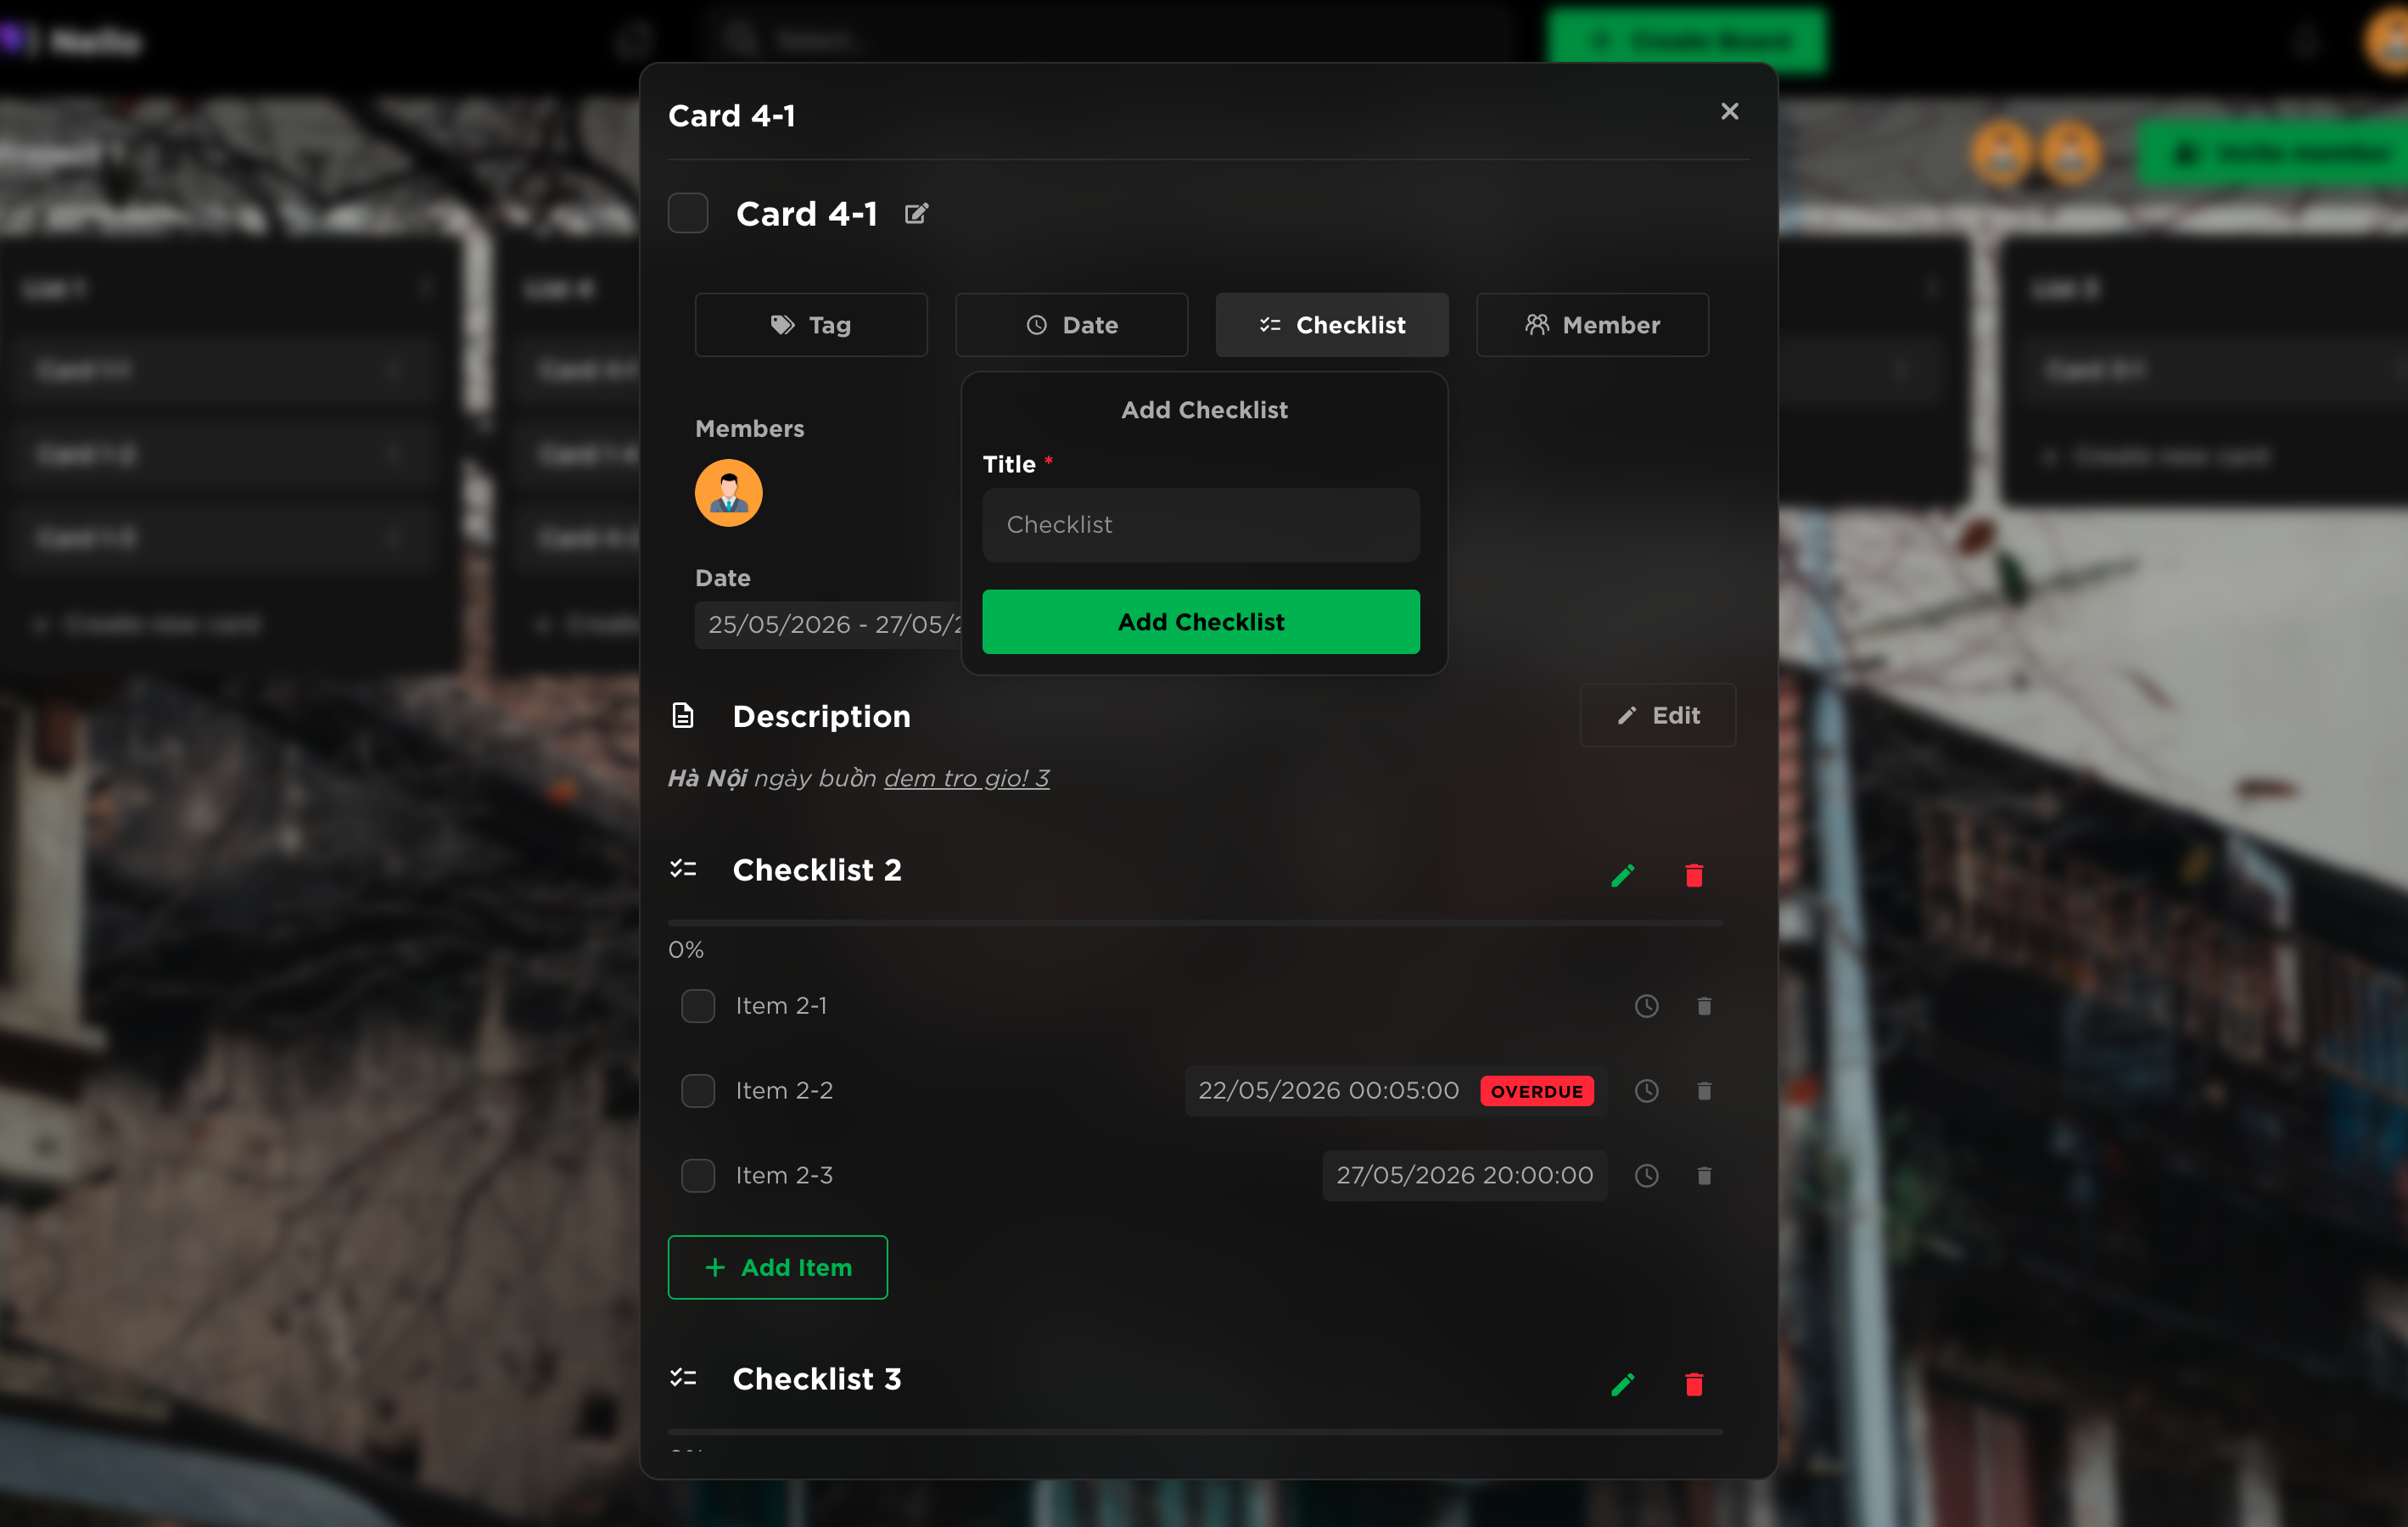
\includegraphics[width=0.9\textwidth]{images/W8_Checklist.png}
\caption{Checklist Management}
\end{figure}

\subsubsection{Card Member}

Đã triển khai chức năng quản lý thành viên được gán cho Card.

Các API đã được tích hợp:

\begin{verbatim}
POST   /api/v1/card-members
DELETE /api/v1/card-members/:id
\end{verbatim}

Các chức năng hỗ trợ:

\begin{itemize}
    \item Gán thành viên vào Card.
    \item Hủy gán thành viên khỏi Card.
    \item Hiển thị danh sách thành viên trong Card Detail.
    \item Hiển thị avatar thành viên trực tiếp trên Card.
\end{itemize}

% TODO: Chèn ảnh Card Member
\begin{figure}[H]
\centering
 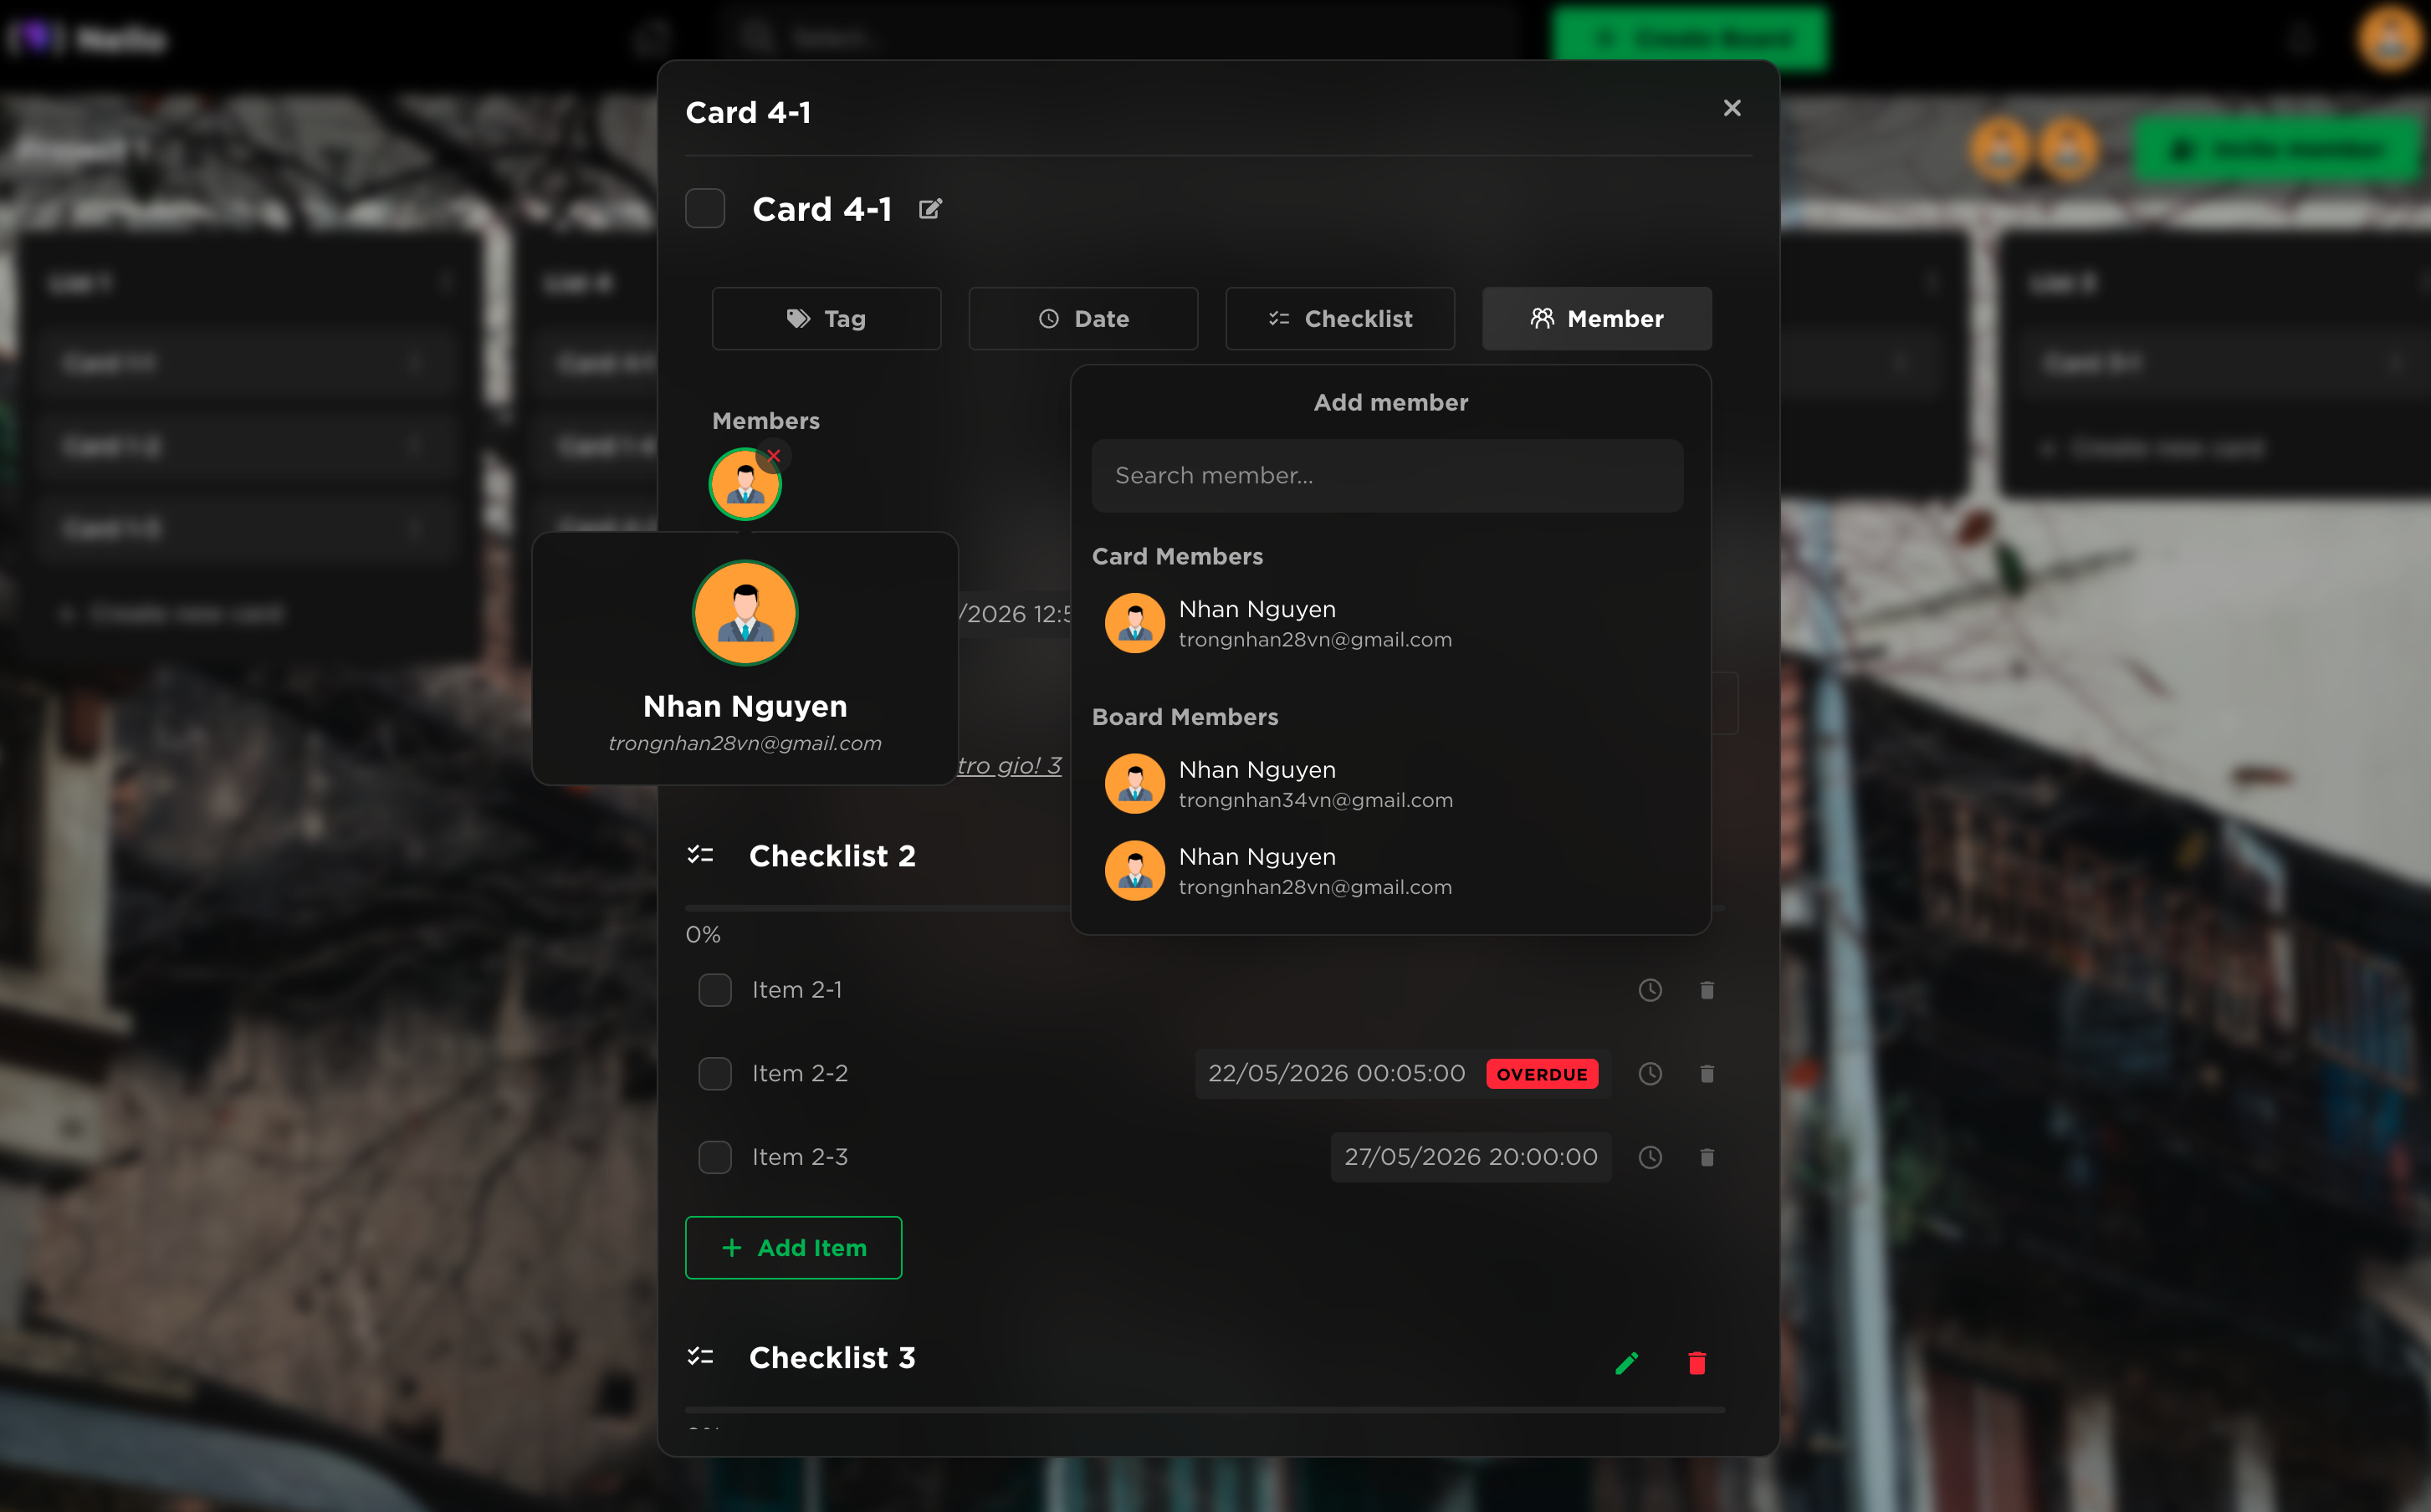
\includegraphics[width=0.9\textwidth]{images/W8_CardMember.png}
\caption{Card Member Management}
\end{figure}

% -------------------------------------------------------
\subsection{Kết luận}
Trong tuần 8, em đã hoàn thành các chức năng trọng tâm còn thiếu của màn
hình Board và Card Detail, bao gồm quản lý thành viên trong Board,
thiết lập Due Date, Checklist và Card Member. Các chức năng đã được tích
hợp đầy đủ với backend API và đảm bảo đồng bộ dữ liệu giữa giao diện và hệ
thống.

Ngoài ra, hệ thống hiện mới được triển khai và kiểm thử trên môi trường
phát triển cục bộ. Việc triển khai lên môi trường Staging vẫn chưa hoàn
thành do cần tiếp tục xử lý một số vấn đề kỹ thuật còn tồn đọng trước khi
đưa hệ thống vào môi trường kiểm thử tập trung.

\clearpage

% ================================================================
\section{CHƯƠNG 2: KẾ HOẠCH PHÁT TRIỂN TRONG GIAI ĐOẠN TIẾP THEO}

\subsection{Bug Drag and Drop}

Hiện vẫn còn tồn tại một số lỗi liên quan đến cơ chế Drag and Drop,
đặc biệt trong các trường hợp kéo thả vào vị trí đầu hoặc cuối danh sách.
Một số thao tác di chuyển Card giữa các List có thể phát sinh sai lệch vị
trí hiển thị giữa Frontend và Backend. Cần tiếp tục rà soát thuật toán xác
định beforeId/afterId và cơ chế cập nhật position.

\subsection{Realtime Websocket}

Hệ thống hiện tại sử dụng cơ chế đồng bộ dữ liệu thông qua API request.
Các thay đổi từ người dùng khác chưa được cập nhật theo thời gian thực.
Cần triển khai Websocket để đồng bộ các sự kiện như tạo Card, cập nhật
Card, thay đổi trạng thái Checklist và Drag and Drop.

\subsection{Phân quyền đối với role VIEWER}

Chức năng phân quyền cho vai trò VIEWER chưa được hoàn thiện.
Hiện tại hệ thống chưa giới hạn đầy đủ các thao tác chỉnh sửa dữ liệu đối
với người dùng chỉ có quyền xem. Cần bổ sung kiểm soát quyền ở cả Frontend
và Backend.

\subsection{Các chức năng mở rộng}

Trong phạm vi thời gian thực hiện Project 1, hệ thống tập trung hoàn thiện các
chức năng cốt lõi phục vụ quản lý công việc theo mô hình Kanban. Một số
tính năng mở rộng vẫn chưa được triển khai và được định hướng phát triển
trong các giai đoạn tiếp theo, bao gồm:

\begin{itemize}
    \item Quản lý nhãn dán (Tag):
    \begin{itemize}
        \item Tạo, chỉnh sửa và xóa Tag.
        \item Gắn nhiều Tag cho Card.
        \item Tìm kiếm và lọc Card theo Tag.
    \end{itemize}

    \item Hệ thống thông báo (Notification):
    \begin{itemize}
        \item Thông báo khi Card được tạo hoặc cập nhật.
        \item Thông báo khi thành viên được gán vào Card.
        \item Thông báo khi công việc sắp đến hạn hoặc quá hạn.
    \end{itemize}

    \item Nhật ký hoạt động (Activity Log):
    \begin{itemize}
        \item Ghi nhận lịch sử tạo, cập nhật và xóa dữ liệu.
        \item Theo dõi lịch sử thay đổi của Board, List và Card.
        \item Hiển thị danh sách hoạt động gần đây của người dùng.
    \end{itemize}
\end{itemize}

\subsection{Triển khai lên môi trường Staging}

Hệ thống hiện mới hoạt động trên môi trường phát triển cục bộ.
Việc triển khai lên môi trường Staging chưa hoàn tất do còn tồn tại một số
lỗi cần xử lý trước khi công bố cho người dùng kiểm thử. Ngoài ra vấn đề
đồng nhất domain giữa Frontend và Backend để hỗ trợ HttpOnly Cookie vẫn
đang được xem xét trong quá trình cấu hình hạ tầng.
